\documentclass[11pt]{article}
\usepackage[a4paper,margin=28mm]{geometry}
\usepackage{amsmath,amssymb,amsthm,mathtools,tikz,booktabs,microtype}
\usepackage[T1]{fontenc}
\usepackage{lmodern}
\usepackage{xurl}
\pdfinfoomitdate=1
\pdftrailerid{}
\pdfsuppressptexinfo=15
\usepackage[colorlinks=true,linkcolor=blue,citecolor=blue,urlcolor=blue,pdfusetitle]{hyperref}
\newtheorem{theorem}{Theorem}[section]
\newtheorem{lemma}[theorem]{Lemma}
\newtheorem{proposition}[theorem]{Proposition}
\newtheorem{corollary}[theorem]{Corollary}
\theoremstyle{remark}
\newtheorem{remark}[theorem]{Remark}
\newcommand{\R}{\mathbb R}
\newcommand{\Z}{\mathbb Z}
\DeclareMathOperator{\area}{area}
\DeclareMathOperator{\diag}{diag}
\DeclareMathOperator{\tr}{tr}
\newcommand{\abs}[1]{\lvert#1\rvert}
\newcommand{\norm}[1]{\lVert#1\rVert}
\newcommand{\BScaling}{Theorem~1.2 of~\cite{RuledApproximation2026}}
\newcommand{\BHyperbolic}{Theorem~1.2 of~\cite{RuledApproximation2026}}
\newcommand{\BLogarithmic}{Corollary~4.4 of~\cite{RuledApproximation2026}}
\newcommand{\BProduct}{Theorem~4.1 of~\cite{RuledApproximation2026}}
\newcommand{\BOrthogonal}{Theorem~1.2 of~\cite{RuledApproximation2026}}
\newcommand{\BNilpotent}{Theorem~1.2 of~\cite{RuledApproximation2026}}
\title{Slope-field perturbations of the two-cylinder covering}
\author{OpenAI}
\date{September 27, 2026}
\begin{document}
\maketitle
\begin{abstract}
The two-cylinder covering of a regular tetrahedron can be perturbed
to give finite covers with total perpendicular base area strictly below
half its minimum projection area. These covers give negative answers
to both the half-area question and the directionwise normalized
half-bound conjecture. By affine invariance, the directionwise
conclusion holds for every nondegenerate tetrahedron.
\end{abstract}
\section{Introduction}\label{c:introduction}

The usual two-cylinder covering of a regular tetrahedron is balanced
at a natural threshold: its total base area is half the tetrahedron's
smallest orthogonal projection area. We ask how the axes can vary across
the two families so as to reduce this cost without leaving a gap.
The answer involves two competing effects. Tilting decreases the
perpendicular area of an intercept patch, but neighboring lines then
need a larger patch to keep covering the tetrahedron. We construct
fields for which the first decrease exceeds the second increase.

A cylinder in $\R^3$ is $B+\R u$, where $u$ is a unit vector and
$B\subset u^\perp$ is measurable with finite planar area $|B|$.
For a convex body $K$, define
\[
 A_{\min}(K)=\min_{|u|=1}|\pi_{u^\perp}K|.
\]
Cylinder covering problems have an antecedent in plank coverings. A plank is the
region between two parallel hyperplanes, and its width is the distance
between them. Bang's plank theorem states that the total width of a
finite plank cover of a convex body is at least the body's minimum width;
Bezdek and Litvak study the corresponding question for
cylinders~\cite[Introduction]{BL2009}.
The half-area question asks whether every finite cylinder cover of $K$
has $\sum_i|B_i|\ge A_{\min}(K)/2$. Bezdek records this question,
and the regular tetrahedron's equality example, as due to
Bang~\cite[Problem~3.1]{Bezdek2009}; the same attribution appears in
Bezdek and Litvak~\cite{BL2009}.

There is a stronger directionwise formulation. For a finite family
$\mathcal C=(B_i+\R u_i)_i$, its relative cost is
\[
 \mathcal R(\mathcal C;K)
   =\sum_i\frac{|B_i|}{|\pi_{u_i^\perp}K|}.
\]
For finite cylinder covers, Bezdek and Litvak proved
$\mathcal R\ge1/3$ for arbitrary
three-dimensional convex bodies and $\mathcal R\ge1$ for ellipsoids
\cite[Theorem~3.1]{BL2009}. Bezdek and Khan's
\emph{1-Codimensional Cylinder Covering Conjecture} proposes
$\mathcal R\ge1/2$ in dimension three
\cite[Definition~3 and Conjecture~4.13]{BK2016}.
Since each denominator is at least $A_{\min}(K)$,
\begin{equation}\label{c:relative-comparison}
 \mathcal R(\mathcal C;K)
 \le\frac{\sum_i|B_i|}{A_{\min}(K)}.
\end{equation}
Thus that conjecture implies the half-area bound. The latter question
is also recorded in Verreault's survey~\cite[Question~4.14]{Verreault2026}.

\begin{theorem}\label{c:main}
Every regular tetrahedron $K\subset\R^3$ of positive edge length admits a finite
cylinder cover with compact parallelogram perpendicular bases such that
\[
 \sum_i|B_i|<\tfrac12 A_{\min}(K),
 \qquad
 \sum_i\frac{|B_i|}{|\pi_{u_i^\perp}K|}<\tfrac12.
\]
It also admits finite covers with bounded open measurable bases
satisfying both inequalities.
\end{theorem}

The directionwise conclusion extends to all tetrahedra. The reason is
the affine invariance of relative cylinder cost, noted by Bezdek and
Litvak~\cite[Section~3]{BL2009}.

\begin{corollary}\label{c:affine-tetrahedra}
Every nondegenerate tetrahedron $T\subset\R^3$ admits a finite cylinder
cover $\mathcal C$ with compact parallelogram perpendicular bases and
$\mathcal R(\mathcal C;T)<1/2$. The same conclusion holds with bounded
open measurable bases.
\end{corollary}
\begin{proof}
Translations preserve all the areas in the relative cost, so consider
an invertible linear map $A$. For a unit vector $u$, put
$v=Au/|Au|$ and define the linear map between perpendicular planes
\[
 Q_u=\pi_{v^\perp}A\big|_{u^\perp}:u^\perp\longrightarrow v^\perp.
\]
It is invertible: if $Q_up=0$, then $Ap$ is parallel to $Au$, so
$p$ is parallel to $u$ and belongs to $u^\perp$, hence is zero.
The image of $B+\R u$ has perpendicular base $Q_uB$, and
$\pi_{v^\perp}(AK)=Q_u(\pi_{u^\perp}K)$. The same positive planar
Jacobian therefore multiplies the numerator and denominator of
$|B|/|\pi_{u^\perp}K|$. Thus the relative cost is unchanged, and the
stated base classes are preserved. Every nondegenerate tetrahedron is
an invertible affine image of a regular one, so Theorem~\ref{c:main}
proves the corollary.
\end{proof}

Together with the lower bound of Bezdek and Litvak, this places the
infimum relative cost of a finite cylinder cover of any nondegenerate
tetrahedron in $[1/3,1/2)$. The absolute half-area inequality in
Theorem~\ref{c:main} concerns regular tetrahedra; the affine argument
preserves each directionwise ratio.

The absolute inequality follows already from the rational field in
Section~\ref{c:rat-rational}; \eqref{c:relative-comparison} gives the
relative inequality for that same cover. The subsequent constructions
explain two further ways to preserve the overlap. They have different
local geometry and different behavior at the apex, even though they
lead to the same strict comparison.

Here is the common construction. A point $p=(p_1,p_2)$ in a planar
label set specifies a segment
\[
 \bigl(s,p_1+sV_1(p),h(p_2+sV_2(p))\bigr),\qquad |s|\le L,
\]
where $h>0$ is a fixed physical scale and $V(p)$ is its slope.
Freezing that slope on an intercept patch of parameter area $A$
gives perpendicular area
\[
 \frac{hA}{\sqrt{1+V_1(p)^2+h^2V_2(p)^2}}.
\]
The scalar product of the unit normals of the intercept plane
$\{x=0\}$ and the plane perpendicular to $(1,V_1(p),hV_2(p))$
gives this projection factor. It suggests an integral cost for a continuously
varying family, but does not by itself produce a finite cover.
The companion article \emph{Finite cylinder approximation of ruled
sets}~\cite[Theorem~1.2]{RuledApproximation2026} provides a finite
square-tile realization for a compact label set $D$ and a field $V$
that is $C^1$ on a neighborhood of $D$ and satisfies
$\operatorname{tr}DV=0$ and $-L^{-2}<\det DV\le0$.
This one construction includes opposite nonzero real eigenvalues
within the strict length bound and square-zero differentials with
unrestricted shear. Its weights use the original velocity coordinates,
and physical base area includes the factor $h$. To obtain a prescribed
physical area error $e$, we use weighted tolerance $e/h$ in the theorem.
We check the relevant conditions only after fixing the field's
regularization or cutoff.

The rational field is derived from a stream function constant on the
two walls of a wedge. A positive denominator makes it smooth at the
apex, while wall tangency makes the tilted straight-line maps preserve
the wedge. The labels assigned to a point by the two complementary
families move in opposite directions to first order. A quartic
enlargement of the label domains leaves a nonnegative square as their
second-order overlap surplus. Its area costs less than the projection
gain. We prove coverage both by comparing two failed inverse labels
and, independently, by locating monotone height thresholds.

The singular power field changes the radial homogeneity. Its derivative
is hyperbolic away from the apex; a cutoff is chosen so that the
differential remains small while two tip cylinders cost less than the
quadratic gain. At the limiting exponent, this field becomes the angular
field with square-zero differential. That endpoint is handled without
a small-shear estimate. It cannot be defined at its apex
by continuity. We remove the apex before applying the companion
theorem and then cover the omitted angular segments by a finite
velocity net.

Section~\ref{c:rat-rational} supplies the first complete construction,
including the strict cost comparison and its finite realization.
Section~\ref{c:rat-threshold} gives the independent threshold proof.
Section~\ref{c:rational-dictionary} relates two coordinate forms of the
rational field and applies the distinct logarithmic-cell and product-cell
approximation theorems. Sections~\ref{c:sing-fields} and
\ref{c:nil-section} develop the singular and square-zero constructions.
The reference area is first computed by projecting entering faces.
Appendix~\ref{c:projection-appendix} gives two further explanations,
through the second moments of a normal frame and the derivative of
translated overlap volume.

\section{A rational field and two choices of padding}
\label{c:rat-rational}

The equality configuration for the regular tetrahedron uses two
edge-parallel cylinders.  We tilt their axes by a smooth field and
slightly enlarge their parameter domains.  The enlargement must be large
enough to preserve coverage but small enough to be paid for by the decrease
in perpendicular projection area.  The construction below makes this
comparison explicit.

Put $h=1/\sqrt2$ and use the regular edge-one tetrahedron
\begin{equation}\label{c:rat-tetrahedron}
 K_1=\{(x,y,ht):-\tfrac12\le t\le\tfrac12,
       \ |x|\le(\tfrac12+t)/2,\ |y|\le(\tfrac12-t)/2\}.
\end{equation}
Throughout this section write $K=K_1$. Its minimum orthogonal projection area is $h/2$.  We verify this using
Cauchy's projection formula for polytopes, obtained by taking support
functions in the projection-body representation
\cite[equation~(1), p.~83, and Section~3]{Martini1991}.  Its volume is $h/6$, by integration
of the rectangular horizontal sections, and its diameter is one.
For a unit vector $u$, let $d_i$ be the derivatives in direction $u$ of
its four affine barycentric coordinates.  Projecting the entering faces
of the tetrahedron gives
\[
 |\pi_{u^\perp}K|=3\operatorname{vol}(K)\sum_{d_i>0}d_i.
\]
Indeed the inward normal component on the face opposite vertex $v_i$
is $d_i$ times that face's altitude; the projected entering faces
partition the shadow except along projected edges.  Write
$s=\sum_{d_i>0}d_i$.  Since $\sum_i d_i=0$ and
$u=\sum_i d_i v_i$, the vector $u/s$ is a difference of two convex
combinations of the vertices.  The diameter bound gives $s\ge1$.
An edge direction has barycentric derivatives $1,-1,0,0$, proving
$A_{\min}(K)=h/2$.

The equality cover can now be specified explicitly. In the label plane
with coordinates $(Y,T)$, put
\[
 D_0=\{(Y,T):0\le T\le\tfrac12,
                        2|Y|\le\tfrac12-T\}.
\]
The triangle $\{(0,Y,hT):(Y,T)\in D_0\}$, swept parallel to the
$x$-axis, covers the portion $t\ge0$. The reflected triangle
$\{(X,0,-hR):(X,R)\in D_0\}$, swept parallel to the $y$-axis,
covers $t\le0$. Each is already perpendicular to its axis and has
area $h\int_0^{1/2}(1/2-T)\,dT=h/8$, so the total cost is $h/4$.
This is the tetrahedral equality configuration attributed to Bang in
Bezdek's account~\cite[Section~3]{Bezdek2009}.

In the label plane with coordinates $(Y,T)$, write $r=\tfrac12-T$ and set
\[
 \mathcal W=\{(Y,T):r\ge2|Y|\}.
\]
The polynomial $Y^2-r^2/4$ vanishes on both wedge walls.
Dividing it by $r$ produces a potential homogeneous of degree one in $(Y,r)$,
whose gradient depends only on the ratio $Y/r$ away from the apex.
Replacing that denominator by $r+d$ smooths the common apex while
retaining the wall values.  Fix $d>0$ and, on $r>-d$, define
\begin{align}
 \psi(Y,T)&=\frac{Y^2-r^2/4}{4(r+d)}, &
 W_d=(a,b)&=(-\psi_T,\psi_Y),\label{c:rat-potential}\\
 a(Y,T)&=-\frac{Y^2}{4(r+d)^2}
          -\frac{r(r+2d)}{16(r+d)^2}, &
 b(Y,T)&=\frac{Y}{2(r+d)}.\label{c:rat-field}
\end{align}
The standard stream-function form makes the divergence zero and the constant
value of $\psi$ on either wedge wall makes the field tangent to that wall.
We use the straight-line maps $p\mapsto p+\epsilon xW_d(p)$,
not a flow of $W_d$.  The exact derivative identities needed later are
\begin{equation}\label{c:rat-spectrum}
 \operatorname{tr}DW_d=0,\qquad
 \det DW_d=-\frac{d^2}{16(r+d)^4}.
\end{equation}
For example, the $YY,Yr,rr$ derivatives of $\psi$ are
$1/[2(r+d)]$, $-Y/[2(r+d)^2]$, and
$(Y^2/2-d^2/8)/(r+d)^3$.  Their determinant is the one displayed;
replacing $r$ by $\tfrac12-T$ preserves it.

At the dividing level $T=0$, put
\begin{align}
 \alpha&=\frac1{1+2d},&
 c(Y)&=c_0+c_2Y^2=-a(Y,0),\notag\\
 c_0&=\frac{(1/2)(1/2+2d)}{16(1/2+d)^2},&
 c_2&=\frac1{4(1/2+d)^2},&
 P(Y)&=\alpha c(Y)Y^2.\label{c:rat-ceiling-polynomial}
\end{align}
Thus $b(Y,0)=\alpha Y$.  For a positive tilt $\epsilon$ and a
positive padding $q=q(\epsilon)$, use the compact label domain
\begin{equation}\label{c:rat-domain}
 D_{\epsilon,q}=\{(Y,T)\in\mathcal W:T\ge-\tfrac14,
                         \ T\ge-\epsilon^2P(Y)-q\}.
\end{equation}
Figure~\ref{c:fig-equality} shows how this domain extends $D_0$
while retaining the wedge walls.

\begin{figure}[htb]
\centering
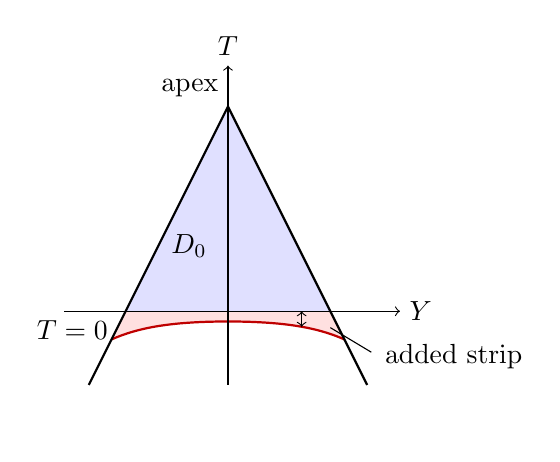
\begin{tikzpicture}[scale=5.2]
 \fill[blue!12] (-.25,0)--(.25,0)--(0,.5)--cycle;
 \begin{scope}
  \clip (-.4,-.3)--(.4,-.3)--(0,.5)--cycle;
  \fill[red!12] (-.34,0)--(.34,0)
    -- plot[domain=.34:-.34,samples=80]
       (\x,{-.025-.3*\x*\x-3*\x*\x*\x*\x}) -- cycle;
  \draw[red!75!black,thick,domain=-.34:.34,samples=80]
    plot (\x,{-.025-.3*\x*\x-3*\x*\x*\x*\x});
 \end{scope}
 \draw[thick] (-.34,-.18)--(0,.5)--(.34,-.18);
 \draw[dashed] (-.25,0)--(.25,0);
 \draw[->] (0,-.18)--(0,.60) node[above] {$T$};
 \draw[->] (-.40,0)--(.42,0) node[right] {$Y$};
 \node[below left] at (-.27,0) {$T=0$};
 \node at (-.095,.16) {$D_0$};
 \node[above left] at (0,.5) {apex};
 \draw[<->] (.18,0)--(.18,-.038);
 \node[right] at (.36,-.11) {added strip};
 \draw[thin] (.35,-.10)--(.25,-.04);
\end{tikzpicture}
\caption{Schematic intercept domain for the first family. The blue
triangle is the unperturbed domain $D_0$; the red strip extends it
below $T=0$. The padded lower boundary ends at the unchanged wedge
walls. Its actual equation is $T=-\epsilon^2P(Y)-q$; the padding is
exaggerated here, and the walls continue below the displayed portion.}
\label{c:fig-equality}
\end{figure}


The two swept sets are
\begin{align}
 S_+&=\{(x,Y+\epsilon xa(Y,T),h(T+\epsilon xb(Y,T))):
                 (Y,T)\in D_{\epsilon,q},\ |x|\le\tfrac12\},\notag\\
 S_-&=\{(X-\epsilon ya(X,R),y,-h(R-\epsilon yb(X,R))):
                 (X,R)\in D_{\epsilon,q},\ |y|\le\tfrac12\}.
 \label{c:rat-sweeps}
\end{align}
For one family, the weighted parameter area is
\begin{equation}\label{c:rat-weighted-cost}
 C_d(\epsilon,q)=h\int_{D_{\epsilon,q}}
          \frac{dY\,dT}{\sqrt{1+\epsilon^2(a^2+h^2b^2)}}.
\end{equation}
This is the quantity in the finite-approximation theorem: the factor $h$
comes from the label plane's physical scale, and the square-root factor
from its orthogonal projection perpendicular to the local line direction.

\begin{proposition}\label{c:rat-rational-proposition}
Fix $d>0$ and a positive function $q(\epsilon)$ such that
$q(\epsilon)=O(\epsilon^2)$ and $\epsilon^3=o(q(\epsilon))$ as
$\epsilon\downarrow0$.  For all sufficiently small $\epsilon>0$,
\[
 K\subset S_+\cup S_-.
\]
Moreover, with
\[
 D_0=\mathcal W\cap\{T\ge0\},\quad
 J_d=\int_{-1/4}^{1/4}P(Y)\,dY,\quad
 I_d=\frac12\int_{D_0}(a^2+h^2b^2)\,dY\,dT,
\]
one has
\begin{equation}\label{c:rat-cost-expansion}
 \frac{C_d(\epsilon,q)}h
   =\frac18+\epsilon^2(J_d-I_d)+\frac q2+O(\epsilon^4).
\end{equation}
The remainder constant may depend on $d$ and on a fixed bound for
$q/\epsilon^2$.  The coverage threshold may also depend on the rate
at which $\epsilon^3/q$ tends to zero.  Finally,
\begin{equation}\label{c:rat-coefficient-limits}
 \lim_{d\downarrow0}J_d=\frac{16}{15360},\qquad
 \lim_{d\downarrow0}I_d=\frac{17}{15360}.
\end{equation}
\end{proposition}

We first establish coverage, including the wedge walls.  We then compare
the area added to the label domain with the area saved by tilting the
axes.  Keeping $d$ fixed throughout these two arguments is essential:
the limiting field at $d=0$ is used only to evaluate coefficient limits.

\subsection{Inverting the tilted maps}
\label{c:rat-inverse}

We first obtain inverse labels anywhere in the wedge; the next
subsection tests their lower-boundary inequalities. For fixed $d$, both
$W_d$ and $DW_d$ are bounded on the entire wedge.
For $|x|\le\tfrac12$, consider
\[
 F_x(Y,T)=(Y,T)+\epsilon xW_d(Y,T).
\]
We claim that $F_x$ maps $\mathcal W$ onto itself for all sufficiently
small $\epsilon$, uniformly in $x$.  The same statement holds with
$-\epsilon$.

The wall functions $r/2\pm Y$ change by
$\epsilon x(-b/2\pm a)$.  Each latter expression vanishes on the
corresponding wall and has bounded $Y$-derivative.  Moving horizontally
from that wall gives
\[
 |-b/2\pm a|\le C_d(r/2\pm Y)\quad\text{on }\mathcal W.
\]
For small $\epsilon$, therefore, each wall function retains its sign
and vanishes precisely on the same wall.  The interior maps into the
interior and the boundary into the boundary.  Also
\[
 \det DF_x=1+\epsilon^2x^2\det DW_d>0
\]
uniformly on the wedge, so the image of its interior is open by the
inverse function theorem.  The image of the closed wedge is closed:
a convergent sequence of images has bounded preimages because the
displacement is bounded, and hence has a convergent subsequence of
preimages in the wedge.  Boundary points cannot map to the interior.
Consequently the interior image is also closed relative to the
connected wedge interior.  It is nonempty, so it is the whole interior;
closedness supplies the boundary.  This proves the claim.

\subsection{Why the two families leave no gap}
\label{c:rat-overlap}

For $(x,y,ht)\in K$, both $(y,t)$ and $(x,-t)$ lie in $\mathcal W$.
The preceding surjectivity supplies wedge labels satisfying
\begin{align*}
 y&=Y+\epsilon xa(Y,T),&t&=T+\epsilon xb(Y,T),\\
 x&=X-\epsilon ya(X,R),&-t&=R-\epsilon yb(X,R).
\end{align*}
If either label belongs to $D_{\epsilon,q}$, the point is covered.
Suppose both labels fail.  Since $P$ and $q$ are nonnegative, this
forces $T,R<0$.  Boundedness of $W_d$ first gives
$|t|,|T|,|R|=O(\epsilon)$ and $Y=y+O(\epsilon)$,
$X=x+O(\epsilon)$.  All remainders below are uniform over $K$.
Since $b(Y,0)=\alpha Y$,
\[
 T=t-\epsilon\alpha xy+O(\epsilon^2),\qquad
 R=-t+\epsilon\alpha xy+O(\epsilon^2).
\]
Their sum is $O(\epsilon^2)$ and both are negative, so separately
$T,R=O(\epsilon^2)$.  The smooth formulas now give
\begin{align*}
 Y&=y+\epsilon xc(y)+O(\epsilon^2),&
 X&=x-\epsilon yc(x)+O(\epsilon^2),\\
 b(Y,T)&=\alpha y+\epsilon\alpha xc(y)+O(\epsilon^2),&
 b(X,R)&=\alpha x-\epsilon\alpha yc(x)+O(\epsilon^2).
\end{align*}
Thus
\begin{equation}\label{c:rat-inverse-sum}
 T+R=-\epsilon^2\alpha\bigl(x^2c(y)+y^2c(x)\bigr)+O(\epsilon^3).
\end{equation}
The choice of $P$ is explained by the exact identity
\begin{equation}\label{c:rat-square-surplus}
 P(x)+P(y)-\alpha\bigl(x^2c(y)+y^2c(x)\bigr)
       =\alpha c_2(x^2-y^2)^2\ge0.
\end{equation}
Replacing $x,y$ by $X,Y$ in $P$ changes it by $O(\epsilon)$.
Equation~\eqref{c:rat-inverse-sum} therefore gives
\[
 T+R\ge-\epsilon^2(P(X)+P(Y))-C\epsilon^3.
\]
The cutoff at $-1/4$ cannot fail when $T,R=O(\epsilon^2)$.
Failure of both remaining domain inequalities would give instead
\[
 T+R<-\epsilon^2(P(X)+P(Y))-2q.
\]
This contradicts $\epsilon^3=o(q)$.  The two families therefore cover
all of $K$, including the boundary points handled by the inverse maps.

\subsection{The area comparison and finite choices}
\label{c:rat-area}

We now prove the cost assertions in Proposition~\ref{c:rat-rational-proposition}.
The unperturbed label domain $D_0$ has area $1/8$.  For
$|Y|\le1/4$, the added interval below $T=0$ has length exactly
$\epsilon^2P(Y)+q$ for small $\epsilon$.  Outside that interval of
$Y$-values, both the width and depth of the added portion are
$O(\epsilon^2)$, because $q=O(\epsilon^2)$ and $P$ is bounded on
$|Y|\le3/8$.  Hence
\[
 |D_{\epsilon,q}|=\frac18+\epsilon^2J_d+\frac q2+O(\epsilon^4).
\]
The field is bounded on these domains.  Taylor expansion of the
integrand in \eqref{c:rat-weighted-cost} has uniform remainder
$O(\epsilon^4)$, and replacing the domain of its quadratic term by
$D_0$ changes that term by $O(\epsilon^4)$.  This proves
\eqref{c:rat-cost-expansion} with its stated remainder.

For the coefficient comparison we may now let $d\downarrow0$.
On $T=0$ one has
$P(Y)\to(1/16+Y^2)Y^2$, giving
\[
 J_d\longrightarrow\int_{-1/4}^{1/4}(Y^2/16+Y^4)\,dY
                 =\frac1{960}.
\]
On $D_0$, write $z=Y/r$ away from the apex.  Then $|z|\le1/2$,
$a\to-(1/16+z^2/4)$ and $b\to z/2$.  The fields are uniformly
bounded there for $d>0$, so bounded convergence and $dY\,dT=r\,dz\,dr$
yield
\[
 I_d\longrightarrow\frac12\int_0^{1/2}r\,dr
     \int_{-1/2}^{1/2}
      \left[\left(\frac1{16}+\frac{z^2}4\right)^2
                     +\frac12\left(\frac z2\right)^2\right]dz
     =\frac{17}{15360}.
\]
This completes the proof of Proposition~\ref{c:rat-rational-proposition}.

There are two useful parameter schedules.  First choose $d>0$ with
$\Delta_d=I_d-J_d>0$.
For \emph{vanishing padding}, take $q=\epsilon^{5/2}$; then
\[
 C_d(\epsilon,\epsilon^{5/2})/h
       =\frac18-\Delta_d\epsilon^2+o(\epsilon^2)<\frac18
\]
for all sufficiently small positive $\epsilon$.
For \emph{fixed quadratic padding}, choose $\eta>0$ with
$\eta/2<\Delta_d$, keep it fixed, and take $q=\eta\epsilon^2$.
In this case the sharper expression is
\[
 C_d(\epsilon,\eta\epsilon^2)/h
       =\frac18-(\Delta_d-\eta/2)\epsilon^2+O(\epsilon^4)<\frac18.
\]
The parameter order is respectively $d,\epsilon$ or $d,\eta,\epsilon$.

For either schedule, fix such a positive $\epsilon$.
The label domain is compact, and the field is smooth on a neighborhood
of it.  The eigenvalues of $D(\pm\epsilon W_d)$ are
\[
 \pm\frac{\epsilon d}{4(r+d)^2}.
\]
Since $d$ was fixed first, their magnitudes times the axial half-length
$1/2$ are strictly below one when $\epsilon$ is small.
Apply \BScaling{} with $V=+\epsilon W_d$
for $S_+$, and with $V=-\epsilon W_d$ followed by the isometry
$(x,y,z)\mapsto(y,x,-z)$ for $S_-$.  Each application gives finitely
many cylinders with cost at most $C_d(\epsilon,q)+e$.  Choose the sum of the two errors less than
$h/4-2C_d(\epsilon,q)>0$.  Together the finite covers cover $K$ and
have total cost less than $h/4=A_{\min}(K)/2$.
The approximation theorem gives compact parallelogram bases.  Enlarging
them slightly in their own perpendicular planes also gives bounded
open parallelogram bases, with the total added area chosen smaller
than the remaining strict slack.  No mesh uniform in $\epsilon$ is
needed.  Similarity scales every base area and the minimum projection
area by the same factor, proving Theorem~\ref{c:main}
for every positive edge length.

\section{A threshold proof for fixed quadratic padding}
\label{c:rat-threshold}

The preceding overlap proof assumes that both labels fail and then
compares their heights.  For fixed quadratic padding there is a second
way to locate the overlap: give an explicit sufficient height for each
family.  This also explains why the same quartic polynomial appears in
both constructions.

Fix $d,\eta>0$ and take $q=\eta\epsilon^2$ in
\eqref{c:rat-domain}.  For $|x|,|y|\le1/2$, put
\begin{equation}\label{c:rat-threshold-function}
 \Theta_x(y)=\epsilon\alpha xy
       +\epsilon^2\bigl(\alpha x^2c(y)-P(y)\bigr).
\end{equation}
We prove the following sufficient condition for the first family:
\begin{equation}\label{c:rat-threshold-inclusion}
 (y,t)\in\mathcal W,\quad -\tfrac12\le t\le\tfrac12,
 \quad t\ge\Theta_x(y)
 \quad\Longrightarrow\quad
 (y,t)=F_x(Y,T)\text{ for some }(Y,T)\in D_{\epsilon,q}.
\end{equation}
All bounds below are uniform in the displayed variables, with $d,\eta$
fixed.

On the rectangle
$\mathcal R=[-1,1]\times[-1,\tfrac12+d/2]$ the field is smooth and
has a finite Lipschitz constant $L_d$.  For small $\epsilon$, the map
\[
 (Y,T)\longmapsto (y,t)-\epsilon xW_d(Y,T)
\]
is a contraction of $\mathcal R$ into itself for
$|y|\le1/2$, $-1/2\le t\le1/2$.
Indeed the target rectangle has positive margins inside $\mathcal R$,
the field is bounded there, and $\epsilon L_d/2<1$.
The inverse label therefore exists and is unique in $\mathcal R$.
The inverse preserves the wedge directly.  Indeed,
\begin{align*}
 -b/2+a&=-(r/2+Y)\frac{2Y+2d+r}{8(r+d)^2},\\
 -b/2-a&=(r/2-Y)\frac{-2Y+2d+r}{8(r+d)^2}.
\end{align*}
The displayed coefficients are bounded on $\mathcal R$.  The target wall
functions $(1/2-t)/2\pm y$ are therefore the corresponding label wall
functions $r/2\pm Y$ multiplied by positive factors when $\epsilon$
is small.  Nonnegativity of the target wall functions implies
nonnegativity of the label wall functions, including equality on either
wall.  Thus this inversion argument does not require the surjectivity
proof in Section~\ref{c:rat-inverse}.

For fixed $x,y$, the inverse height $T$ increases strictly with $t$.
In fact if the target heights differ by $\Delta t>0$, and $p,p'$
are their inverse labels, then
\[
 |(p'-p)-(0,\Delta t)|\le\frac{\epsilon L_d}{2}|p'-p|
 \le\frac{\epsilon L_d/2}{1-\epsilon L_d/2}\,\Delta t.
\]
The last coefficient is less than one for small $\epsilon$.
At $t=\Theta_x(y)$, the inverse equations first give
$Y=y+O(\epsilon)$ and $T=O(\epsilon)$.
Using $b(y,0)=\alpha y$ improves the latter bound to
$T=O(\epsilon^2)$.  Consequently
\[
 Y=y+\epsilon xc(y)+O(\epsilon^2),\qquad
 b(Y,T)=\alpha y+\epsilon\alpha xc(y)+O(\epsilon^2),
\]
and substitution in the height equation gives
\[
 T=-\epsilon^2P(y)+O(\epsilon^3)
   =-\epsilon^2P(Y)+O(\epsilon^3).
\]
The rectangle inversion also applies at the threshold if
$(y,\Theta_x(y))$ lies outside the wedge.  Boundedness of the field
on $\mathcal R$ gives $Y=y+O(\epsilon)$ uniformly over the entire
target height interval, not only at the threshold.  Thus changing from
the threshold label to any of these labels changes $P(Y)$ by
$O(\epsilon)$.  Combining this bound with monotonicity gives, for all
$t\ge\Theta_x(y)$ under consideration,
\[
 T\ge-\epsilon^2P(Y)-C\epsilon^3
       \ge-\epsilon^2P(Y)-\eta\epsilon^2,
 \qquad T\ge-\tfrac14
\]
when $\epsilon$ is sufficiently small.
The inverse label is in the wedge, proving
\eqref{c:rat-threshold-inclusion}.

Applying the same argument with $x$ replaced by $-y$ gives a sufficient
condition $-t\ge\Theta_{-y}(x)$ for the second family.  But
\[
 \Theta_x(y)+\Theta_{-y}(x)
   =-\epsilon^2\alpha c_2(x^2-y^2)^2\le0.
\]
At least one of those two conditions holds for every point of $K$.
This proves coverage again.  The fixed positive $\eta$ absorbs the
uniform cubic inverse error; the area calculation in
Section~\ref{c:rat-area} then shows how small $\eta$ must be chosen
before fixing $\epsilon$.

\section{Two coordinate forms and two finite realization methods}
\label{c:rational-dictionary}

The rational construction already gives a finite cover with a strict
area saving.  We now express the same geometry in fully orthonormal
coordinates and compare two other ways to obtain its finite cylinders.
The coordinate change tracks the slope, quartic padding, and
perpendicular area together.  In these coordinates the logarithmic-cell
theorem gives bounded open bases; in the centered coordinates the
product-cell theorem does so under a weaker smoothness assumption.
All three methods approximate the same weighted integral cost to
arbitrary additive accuracy, but their hypotheses and base shapes differ.

Put $c_*=1/\sqrt2$ and
\begin{equation}\label{c:uncentered-tetrahedron}
 K_0=\{(x_0,y_0,z_0):0\le z_0\le2,
          |y_0|\le c_*z_0,\ |x_0|\le c_*(2-z_0)\}.
\end{equation}
It is a regular tetrahedron of edge $2\sqrt2$. For a fixed
$d_0>0$, define on $s>-d_0$
\begin{align}
 g(s)&=\frac{1+d_0}{s+d_0},\notag\\
 v_1(u,s)&=c_*^2s g(s)+\tfrac12(c_*^2s^2-u^2)g'(s),
 &v_2(u,s)&=u g(s).\label{c:uncentered-field}
\end{align}
This is the stream-function field associated with
$g(s)(u^2-c_*^2s^2)/2$. In particular it is tangent to
$u=\pm c_*s$. Let
\begin{align}
 A_0&=c_*^2\left(1-\frac1{2(1+d_0)}\right),&
 B_0&=\frac1{2(1+d_0)},\notag\\
 a_0(u)&=A_0u^2+B_0u^4=u^2v_1(u,1),\label{c:uncentered-polynomial}\\
 U_k&=\{(u,s):0\le s\le3/2, |u|\le c_*s,
                   s\le1+k^2(a_0(u)+\eta_0)\},\notag
\end{align}
where $\eta_0>0$ will be fixed before the tilt $k>0$.
For $|r|\le2c_*$, write $F_r(p)=p+rk v(p)$. The two swept sets are
\begin{align}
 E_1&=\{(x_0,y_0,z_0):|x_0|\le2c_*, (y_0,z_0)\in F_{x_0}(U_k)\},\notag\\
 E_2&=\{(x_0,y_0,z_0):|y_0|\le2c_*, (x_0,2-z_0)\in F_{-y_0}(U_k)\}.
 \label{c:uncentered-sweeps}
\end{align}

\begin{proposition}\label{c:rational-coordinate-identity}
Let $\ell=1/(2\sqrt2)$ and define the Euclidean similarity
\[
 \Phi(x_0,y_0,z_0)=(-\ell x_0,\ell y_0,\ell(1-z_0)).
\]
Then $\Phi K_0=K_1$, and the two sets in
\eqref{c:uncentered-sweeps} are carried exactly to the two sets in
\eqref{c:rat-sweeps} with
\begin{equation}\label{c:rational-parameter-dictionary}
 d=d_0/2,\qquad \epsilon=4(1+d_0)k,
 \qquad q=\eta_0 k^2/2.
\end{equation}
In particular $q=\eta\epsilon^2$ where
$\eta=\eta_0/[32(1+d_0)^2]$. All perpendicular areas are multiplied
by $1/8$.
\end{proposition}
\begin{proof}
Write $(Y,T)=(\ell u,(1-s)/2)$, so $r=s/2$.
Substitution into \eqref{c:rat-field} gives
\begin{equation}\label{c:rational-field-dictionary}
 v_1(u,s)=-4(1+d_0)a(Y,T),\qquad
 v_2(u,s)=2\sqrt2(1+d_0)b(Y,T).
\end{equation}
At $s=1$, these identities and
$\alpha=(1+d_0)^{-1}$ give
\[
 P(\ell u)=\frac{a_0(u)}{32(1+d_0)^2}.
\]
Consequently the last inequality defining $U_k$ is exactly
$T\ge-\epsilon^2P(Y)-q$, and $s\le3/2$ is $T\ge-1/4$.
The wedge inequalities correspond as well. For the first family,
$x=-\ell x_0$ converts its two coordinate equations into
$y=Y+\epsilon x a(Y,T)$ and $t=T+\epsilon x b(Y,T)$.
For the second, take $(X,R)=(-\ell u,(1-s)/2)$ and use that $a$
is even and $b$ is odd in the first coordinate. This gives precisely
the second equation in \eqref{c:rat-sweeps}. The bounds on the free
coordinate become $|x|,|y|\le1/2$.
Finally, $\Phi$ is an isometry followed by dilation by $\ell$;
it multiplies every perpendicular area by $\ell^2=1/8$.
\end{proof}

The monotone thresholds in Section~\ref{c:rat-threshold} therefore
give, in these coordinates, the sufficient condition
\begin{equation}\label{c:uncentered-threshold}
 z_*\le 1+kr u+k^2\bigl(a_0(u)-r^2v_1(u,1)\bigr)
       \quad\Longrightarrow\quad (u,z_*)\in F_r(U_k),
\end{equation}
provided $0\le z_*\le2$ and $|u|\le c_*z_*$.
The two right-hand thresholds sum to
$2+k^2 B_0(x_0^2-y_0^2)^2\ge2$.
Thus the exact transformation preserves both the bounded contraction
argument and the nonnegative overlap surplus, including the wedge
walls.

\subsection{Logarithmic-cell realization of the fixed-padding cover}

For the field \eqref{c:uncentered-field}, direct differentiation gives
\begin{equation}\label{c:uncentered-spectrum}
 \tr Dv=0,\qquad
 \det Dv=-c_*^2\left(\frac{(1+d_0)d_0}{(s+d_0)^2}\right)^2<0.
\end{equation}
The determinant simplification uses $gg''/2=(g')^2$.
For fixed $d_0$, the field is $C^2$ on an open rectangle containing
$U_k$ for every sufficiently small $k$. The boundary of $U_k$ has
area zero, since it lies in finitely many lines and a polynomial graph.
The strict spectral condition
$2c_* k\sqrt{-\det Dv}<1$ also holds there for small $k$.
These are exactly the hypotheses of \BLogarithmic{}.
It supplies finite covers of each set in \eqref{c:uncentered-sweeps}
with bounded open measurable bases, at cost arbitrarily close from above to
\begin{equation}\label{c:logarithmic-cost}
 J_k=\int_{U_k}(1+k^2|v(u,s)|^2)^{-1/2}\,du\,ds.
\end{equation}
The second application uses $-v$ and an isometry.

The exact cost comparison can also be checked in these coordinates.
Put $U_0=\{0\le s\le1, |u|\le c_*s\}$, of area $c_*$.
The same strip calculation as in Section~\ref{c:rat-area} gives
\begin{equation}\label{c:uncentered-cost}
 J_k=c_*+k^2\left\{
 \int_{-c_*}^{c_*}(a_0(u)+\eta_0)\,du
 -\tfrac12\int_{U_0}|v|^2\right\}+O(k^4).
\end{equation}
For fixed $d_0,\eta_0$, the added horizontal and vertical extensions
are $O(k^2)$; their product is the fourth-order boundary remainder.
Letting $d_0\downarrow0$ only in the coefficient integrals, and setting
$u=sb$, gives
\begin{align*}
 \tfrac12\int_{U_0}|v|^2&\longrightarrow
 \frac14\int_{-c_*}^{c_*}
       \left[\frac{(c_*^2+b^2)^2}{4}+b^2\right]db
       =\frac{c_*^3}{6}+\frac{7c_*^5}{30},\\
 \int_{-c_*}^{c_*}a_0(u)\,du&\longrightarrow\frac{8c_*^5}{15}.
\end{align*}
Bounded convergence is valid because $|u|\le c_*s$ bounds the fields
uniformly for $0<d_0<1$. The first limit exceeds the second by
$c_*^3/60>0$. Choose $d_0>0$ such that the actual difference
\[
 \Delta(d_0)=\tfrac12\int_{U_0}|v|^2
                  -\int_{-c_*}^{c_*}a_0(u)\,du
\]
is positive. Then choose $0<\eta_0<\Delta(d_0)/(2c_*)$,
and finally $k$ small. Formula~\eqref{c:uncentered-cost}
gives $J_k<c_*$. Only then choose the two finite errors with sum
less than $2(c_*-J_k)$. The resulting finite open-base cover has
cost below $2c_*=A_{\min}(K_0)/2$.

The $C^2$ rectangle and strict spectral inequality give the open-base
conclusion directly in the orthonormal $(u,s)$ coordinates.
The scaling identity gives
$C_d(\epsilon,q)=J_k/8$, in agreement with
Proposition~\ref{c:rational-coordinate-identity}.

\subsection{Product-cell realization of the centered cover}

For $q=\epsilon^{5/2}$, use the original centered label set
$D_{\epsilon,q}$ and the two slopes $V=\pm\epsilon W_d$.
The set is compact with area-zero boundary, $V$ is $C^1$ on an open
neighborhood, and $DV$ has eigenvalues
$\pm\epsilon d/[4(r+d)^2]$. With $M=1/2$ and $h=1/\sqrt2$,
the strict condition $0<M\lambda<1$ follows after fixing $d>0$
and taking $\epsilon$ sufficiently small. Therefore \BProduct{}
gives each family a finite cover with bounded open measurable bases
and cost at most $C_d(\epsilon,\epsilon^{5/2})+e$.

The product-cell proof chooses its padding, product threshold, and
local scale in that order, exhausts the interior by disjoint cells,
and covers the remaining null set before taking a finite open subcover.
These approximation choices occur after the present geometric
parameters are fixed. By \eqref{c:rat-cost-expansion}, choose $d$
with $I_d>J_d$, then $\epsilon$ so that $C_d<h/8$, and finally
the two errors with sum below $h/4-2C_d$. This gives the asserted
open-base cover without altering either the fractional padding or
the weighted physical metric. The compact parallelogram construction
in Section~\ref{c:rat-area} remains an independent finite realization
of the same swept sets.

\section{A singular power-law field}
\label{c:sing-fields}

The rational field smooths the common tip before tilting the lines.  We now
keep a power-law singularity in the derivative and remove a small tip
region instead.  Two triangular-base cylinders cover the removed regions;
their cost is smaller than the quadratic saving from the tilted families.
The exponent of the power law makes both requirements compatible.
We give the construction at edge length two, where the cone walls have
slopes $\pm1$, and then state its exact edge-one form.

We use the regular tetrahedron of edge length $2$,
\[
 K_2=\{(x,y,\sqrt{2}\,t):0\le t\le1,
                 \ |x|\le1-t,\ |y|\le t\}.
\]
The physical metric in these coordinates is $dx^2+dy^2+2\,dt^2$.
The minimum projection area is
$A_{\min}(K_2)=4A_{\min}(K_1)=\sqrt2$, since these regular tetrahedra
are related by a similarity of ratio two.  Appendix~\ref{c:projection-appendix}
gives two independent proofs of this normalization.

\begin{theorem}\label{c:sing-theorem}
For every
\[
 1<p<(\sqrt{51}-5)/2,\qquad 1<\gamma<1/(2-p),
\]
all sufficiently small positive $c$ determine a finite cylinder cover
of the regular edge-$2$ tetrahedron $K_2$ above with total perpendicular
base area less than $\sqrt2/2$.  The cover consists of two finite
families with compact parallelogram bases and two cylinders with
compact triangular bases.  Before the arbitrarily small errors needed
for the two finite approximations, the area bound is
\[
 \frac{\sqrt2}{2}+2\sqrt2\,\kappa_p c^2+o(c^2),
 \qquad
 \kappa_p=\frac{(1/2)^4(2p^2+10p-13)}{30p}<0.
\]
The asymptotic statement fixes $p$ and $\gamma$ first.  Each finite
approximation is chosen after the positive value of $c$ is fixed.
\end{theorem}

Put $a=1/2$.  The two cylinders obtained by splitting at $t=a$,
with axes parallel to the $x$- and $y$-axes respectively, have total
base area $2\sqrt{2}\,a^2=\sqrt{2}/2$.  We perturb those directions.

\subsection{The field and the cutoff}

Fix parameters in the order
\begin{equation}
 1<p<\frac{\sqrt{51}-5}{2},\qquad
 1<\gamma<\frac1{2-p},\qquad
 d=c^\gamma\quad(c>0).
 \label{c:sing-parameters}
\end{equation}
The upper bound on $p$ makes the quadratic area coefficient negative.
The bounds on $\gamma$ make the derivative of the tilted field uniformly
small while keeping the tip area $o(c^2)$.
Only $c$ will tend to zero.  To obtain a field tangent to the cone walls
$b=\pm r$, take a stream function that vanishes on both walls.
Multiplying $b^2-r^2$ by $r^{p-2}$ makes the stream function homogeneous
of degree $p$, so the resulting field has degree $p-1$.  The normalization
below also gives $Q(b,a)=b$, which will cancel the first-order overlap terms.
For $r>0$, define
\begin{align}
 \psi(b,r)&=\frac12(r/a)^{p-2}(b^2-r^2),
 &V=(P,Q)&=(-\partial_r\psi,\partial_b\psi),\notag\\
 P(b,r)&=\frac a2(r/a)^{p-1}
       \left[p+(2-p)(b/r)^2\right],
 &Q(b,r)&=(r/a)^{p-2}b.
 \label{c:sing-field}
\end{align}
At the dividing level let
\begin{equation}
 P_a(b)=P(b,a)=\frac{ap}{2}+\frac{2-p}{2a}b^2,
 \qquad \delta(b)=b^2P_a(b).
 \label{c:sing-ceiling-polynomial}
\end{equation}
Thus $\delta\ge0$, $Q(b,a)=b$, and $Q=\pm P$ on $b=\pm r$.
Our compact label domain is
\begin{equation}
 D_c=\{(b,r):d\le r\le2,\ |b|\le r,
                  \ r\le a+c^2\delta(b)+c^{5/2}\}.
 \label{c:sing-domain}
\end{equation}

The field is smooth on $r>0$, and direct differentiation gives
\begin{equation}
 \operatorname{tr}DV=0,\qquad
 \det DV=(r/a)^{2p-4}\frac{p-1}{2}
               \left[(2-p)(b/r)^2-p\right]<0
 \quad (|b|\le r).
 \label{c:sing-hyperbolicity}
\end{equation}
Indeed the determinant equals $\det D^2\psi$; the bracket is at most
$2-2p<0$.  On this cone,
$\|DV(b,r)\|\le C r^{p-2}$, with $C$ depending only on the fixed
parameters.  Consequently
\begin{equation}
 c\sup_{D_c}\|DV\|\le Cc d^{p-2}
   =C c^{1-\gamma(2-p)}\longrightarrow0,
 \qquad d^2=o(c^2).
 \label{c:sing-cutoff-estimates}
\end{equation}
Thus, for sufficiently small $c$, both $cDV$ and $-cDV$ have
eigenvalues $\lambda,-\lambda$ with $0<\lambda<1$ at every label.
Although no derivative bound is asserted at $r=0$, each fixed $D_c$
has a neighborhood on which the field is smooth.

Write $s=1-t$.  Consider the two sets of segments
\begin{align}
 E_c^-&=\{(x,y,\sqrt{2}\,t): |x|\le1,
            \ (y,t)=(b,r)+cxV(b,r),\ (b,r)\in D_c\},\notag\\
 E_c^+&=\{(x,y,\sqrt{2}\,t): |y|\le1,
            \ (x,s)=(b,r)-cyV(b,r),\ (b,r)\in D_c\}.
 \label{c:sing-families}
\end{align}
We apply \BScaling{} with $h=\sqrt{2}$ and $L=1$ to the first
family with field $cV$.
Interchanging $x,y$ and
reflecting and translating the physical height gives the second family
with field $-cV$.  Thus, for each fixed sufficiently small $c$ and any
$e>0$, each family has a finite cylinder cover with compact
parallelogram bases and total base area at most
\begin{equation}
 J(c)+e,
 \qquad
 J(c)=\sqrt{2}\int_{D_c}
       \frac{db\,dr}{\sqrt{1+c^2(P^2+2Q^2)}}.
 \label{c:sing-cost-integral}
\end{equation}
The factor $2$ multiplying $Q^2$ records the physical height scale.

These two applications use the companion's single square-tile
construction. For the fixed compact cutoff domain $D_c$, the fields
$\pm cV$ are $C^1$ on a neighborhood. Equations
\eqref{c:sing-hyperbolicity} and \eqref{c:sing-cutoff-estimates}
give $\operatorname{tr}D(\pm cV)=0$ and
$-1<\det D(\pm cV)<0$ for sufficiently small $c$, which is the
theorem's condition for $L=1$. The tile orientations may vary, but
their weights use the velocities in the original $(b,r)$ coordinates,
giving \eqref{c:sing-cost-integral} with the physical factor $\sqrt2$.
No condition on the area of $\partial D_c$ or smallness of the
operator norm is required by the theorem. The separate cylinders
introduced next cover the omitted tips.


We add an $x$-parallel cylinder with triangular base
$\{(0,y,\sqrt{2}\,t):0\le t\le2d,\ |y|\le t\}$,
and the analogous $y$-parallel cylinder at the upper end, obtained by
projecting $\{0\le s\le2d,\ |x|\le s\}$ to the plane $y=0$.
Each base has area
\begin{equation}
 \sqrt{2}\int_0^{2d}2r\,dr
       =\sqrt{2}(2d)^2.
 \label{c:sing-tip-cost}
\end{equation}

\subsection{Inversion, including the cone boundary}

All estimates below are uniform over the points under consideration,
with $p$ and $\gamma$ fixed.  Suppose
\[
 2d\le T\le1,\qquad |B|\le T,\qquad |k_0|\le c.
\]
We first solve
\begin{equation}
 (B,T)=(b,r)+k_0V(b,r)
 \label{c:sing-inverse}
\end{equation}
without imposing the last inequality of \eqref{c:sing-domain}.
In the closed Euclidean ball of radius $T/4$ about $(B,T)$, one has
$3T/4\le r\le5T/4$ and $|b|/r\le5/3$.  Formula
\eqref{c:sing-field} gives bounds
$|V|\le C T^{p-1}$ and $\|DV\|\le C T^{p-2}$ throughout the ball.
The map
\[
 (b,r)\longmapsto(B,T)-k_0V(b,r)
\]
maps this ball into itself and is a contraction for all sufficiently
small $c$, since $cT^{p-2}\le c(2d)^{p-2}=o(1)$.
Its fixed point satisfies $d\le r\le2$.

To prove that this fixed point lies in the cone, use the exact identities
\begin{equation}
 Q(b,r)\pm P(b,r)
   =\frac{r\pm b}{2}(r/a)^{p-2}
                      \left[(2-p)b/r\pm p\right].
 \label{c:sing-wall-factorization}
\end{equation}
Equation~\eqref{c:sing-inverse} consequently gives
\[
 T\pm B=(r\pm b)(1+\theta_\pm),\qquad
 |\theta_\pm|\le Cc r^{p-2}=o(1).
\]
The factors $1+\theta_\pm$ are positive.  Since $T\pm B\ge0$, we
obtain $r\pm b\ge0$.  This also handles equality on either wall:
no boundary point is lost in passing to inverse labels.

\subsection{The two families overlap sufficiently}

Take a point of $K_2$ outside the two tip regions, so that
$t,s\ge2d$.  Apply \eqref{c:sing-inverse} to $(B,T)=(y,t)$
with $k_0=cx$, and to $(B,T)=(x,s)$ with $k_0=-cy$.
Let the resulting labels be $(b_-,r_-)$ and $(b_+,r_+)$.
They already satisfy $d\le r_\pm\le2$ and $|b_\pm|\le r_\pm$.
It remains to show that one label satisfies its ceiling in
\eqref{c:sing-domain}.

Suppose both ceilings fail.  Since $\delta\ge0$, this implies
$r_-,r_+>a$.  The inverse equations give
\begin{align}
 b_-&=y-cxP(b_-,r_-),&
 b_+&=x+cyP(b_+,r_+),\notag\\
 r_-+r_+&=1+c\left[yQ(b_+,r_+)-xQ(b_-,r_-)\right].
 \label{c:sing-inverse-sum}
\end{align}
All labels now lie in a fixed compact region with $r\ge a$, on which
the field and its derivatives are bounded.  The last equation first
gives $r_-+r_+=1+O(c)$.  Because both summands exceed $a=1/2$,
each is $a+O(c)$.  The first two equations also give
$b_-=y+O(c)$ and $b_+=x+O(c)$.
Using $Q(b,a)=b$, the bracket in the last equation is therefore
$yx-xy+O(c)=O(c)$.  This improves the sum to $1+O(c^2)$ and
each height to $a+O(c^2)$.

Refining the first two equations and again using $Q(b,a)=b$, we obtain
\[
 b_-=y-cxP_a(y)+O(c^2),\qquad
 b_+=x+cyP_a(x)+O(c^2),\qquad
 Q(b_\pm,r_\pm)=b_\pm+O(c^2).
\]
Substitution into \eqref{c:sing-inverse-sum} yields
\begin{equation}
 r_-+r_+
   =1+c^2\left[x^2P_a(y)+y^2P_a(x)\right]+O(c^3).
 \label{c:sing-overlap-expansion}
\end{equation}
On the other hand, failure of both ceilings gives
\[
 r_-+r_+>
  1+c^2\left[\delta(b_-)+\delta(b_+)\right]+2c^{5/2}.
\]
Here $\delta(b_-)+\delta(b_+)=\delta(y)+\delta(x)+O(c)$, and
\begin{align*}
 \delta(y)+\delta(x)-x^2P_a(y)-y^2P_a(x)
  &=(x^2-y^2)\left[P_a(x)-P_a(y)\right]\\
  &=\frac{2-p}{2a}(x^2-y^2)^2\ge0.
\end{align*}
Comparison with \eqref{c:sing-overlap-expansion} would force
$2c^{5/2}\le Cc^3$, which is impossible for sufficiently small $c$.
Thus every middle-region point belongs to $E_c^-\cup E_c^+$.
Together with the two closed tip cylinders, the two families cover
all of $K_2$.

\subsection{The exact quadratic saving}

Let
\[
 H=\{(b,r):0<r\le a,\ |b|\le r\},\qquad |H|=a^2.
\]
The deletion of $r<d$ removes area $d^2=o(c^2)$.  The area added
above $r=a$ is
\[
 c^2\int_{-a}^{a}\delta(b)\,db+o(c^2).
\]
Indeed, for $|b|\le a$ its thickness is exactly
$c^2\delta(b)+c^{5/2}$.  Since $|b|\le r\le2$ and $\delta$ is
bounded there, the remaining portion has $a<|b|\le a+O(c^2)$
and thickness $O(c^2)$, hence area $O(c^4)$.
The field is uniformly bounded on $|b|\le r\le2$ because $p>1$.
Taylor expansion of the integrand in
\eqref{c:sing-cost-integral} therefore has uniform remainder
$O(c^4)$.  Also $|D_c\mathbin{\triangle}H|\to0$, so the bounded
quadratic coefficient may be integrated over $H$.  Including one
tip cylinder, we conclude that
\begin{equation}
 \frac{J(c)}{\sqrt{2}}+4d^2
  =a^2+c^2\kappa_p+o(c^2),\qquad
 \kappa_p=\int_{-a}^a\delta(b)\,db
                -\frac12\int_H(P^2+2Q^2)\,db\,dr.
 \label{c:sing-area-expansion}
\end{equation}

Both terms admit elementary evaluations.  The first is
\[
 \int_{-a}^a\delta(b)\,db
   =a^4\left(\frac p3+\frac{2-p}{5}\right)
   =\frac{2a^4(p+3)}{15}.
\]
For the second, put $\eta=b/r$.  Then
\[
 P=\frac a2(r/a)^{p-1}[p+(2-p)\eta^2],\qquad
 Q=a(r/a)^{p-1}\eta,\qquad db\,dr=r\,d\eta\,dr.
\]
It follows that
\begin{align*}
 \frac12\int_H(P^2+2Q^2)\,db\,dr
 &=\frac{a^4}{4p}\int_{-1}^{1}
          \left\{\frac14[p+(2-p)\eta^2]^2+2\eta^2\right\}\,d\eta\\
 &=\frac{a^4(2p^2+2p+13)}{30p}.
\end{align*}
Thus the exact coefficient is
\begin{equation}
 \boxed{\displaystyle
 \kappa_p=\frac{a^4(2p^2+10p-13)}{30p}<0.}
 \label{c:sing-coefficient}
\end{equation}
The range of $p$ in \eqref{c:sing-parameters} is precisely the
range above $1$ on which this expression is negative.  At $p=1$
its continuous extension is $-a^4/30$; the construction itself uses
$p>1$ to retain strict hyperbolicity.

\paragraph{Completion with finitely many cylinders.}
We can now finish the proof of Theorem~\ref{c:sing-theorem}.  First fix $p$ in the stated
range and then $\gamma$ in \eqref{c:sing-parameters}.
Choose a positive $c$ small enough for the derivative bounds, all
coverage statements, and
\[
 2J(c)+8\sqrt{2}\,d^2
  =\frac{\sqrt{2}}2+2\sqrt{2}\,\kappa_p c^2+o(c^2)
  <\frac{\sqrt{2}}2.
\]
Call the strict difference $\Delta>0$.
Only after fixing this $c$ do we apply
\BScaling{} to each family, choosing
its additive error less than $\Delta/4$.
Those two finite covers and the two triangular tip cylinders give
an actual finite cover of $K_2$ whose total base area is strictly less
than $A_{\min}(K_2)/2$.  The main bases are compact parallelograms.
No uniform choice of their meshes as $c\to0$ is needed.

\subsection{Edge-one normalization and alternative cutoffs}
\label{c:sing-edge-one}

The edge-one form allows a direct comparison with the rational field.
First we transport the whole construction by a similarity; then we explain
which cutoff and padding may be changed without changing its quadratic
saving.  The similarity halves physical lengths while leaving the height
label unchanged:
\[
 (x,y,\sqrt{2}\,t)\longmapsto(y/2,x/2,t/\sqrt{2}),
 \qquad (w,l)=(b/2,r),\qquad k=4c.
\]
Put $h=1/\sqrt{2}$ and define
\[
 \widehat V_1(w,l)=\tfrac14P(2w,l),\qquad
 \widehat V_2(w,l)=\tfrac12Q(2w,l),\qquad
 f(w)=w^2\widehat V_1(w,1/2).
\]
Equivalently, $\widehat V=(-\partial_lH_*,\partial_wH_*)$ for
$H_*(w,l)=2^{p-3}(w^2l^{p-2}-l^{p}/4)$.
The two segment families transform exactly, and
\[
 k^2(\widehat V_1^2+h^2\widehat V_2^2)
     =c^2(P^2+2Q^2),\qquad
 c^2\delta(2w)=k^2 f(w).
\]
With $S=\operatorname{diag}(1/2,1)$, the derivative identity is
\[
 \widehat V=\tfrac12 S V\circ S^{-1},\qquad
 \tfrac12 kD\widehat V=cS(DV)S^{-1}.
\]
Thus the scaled eigenvalues for axial half-length $L=1/2$ agree
with those of $cDV$.  Under the fixed physical rescaling, the derivative is likewise
similar to $\pm kD\widehat V$.
This is a spectral statement; the nonorthogonal matrix $S$ does not
preserve the ordinary operator norm. No operator-norm transfer is needed
by the square-tile theorem. The already constructed physical cylinder
cover also transports by the Euclidean similarity above.

Physical areas scale by $1/4$.  Therefore the per-family quadratic
coefficient after dividing physical area by $h$ is $\kappa_p/32$;
the positive saving in that normalization is
\[
 -\frac{\kappa_p}{32}
   =\frac{13-10p-2p^2}{15360p}.
\]
For this exact similarity the cutoff becomes $4^{-\gamma}k^\gamma$
and the ceiling padding becomes $k^{5/2}/32$.

The estimates also permit independent choices of these two auxiliaries.
Indeed, the preceding inverse, overlap, and area proofs hold with a
positive cutoff $\rho(c)$ and padding $q(c)>0$ whenever
\begin{equation}
 \rho(c)=o(c),\qquad c\rho(c)^{p-2}\longrightarrow0,
 \qquad q(c)=o(c^2),\qquad c^3=o(q(c)).
 \label{c:sing-cutoff-flexibility}
\end{equation}
The contraction and wall-sign estimates use only the second condition;
the deleted label area and two tip areas use the first.  The overlap
contradiction compares $2q(c)$ with $O(c^3)$, and the coefficient is
unchanged because $q(c)=o(c^2)$.  On the retained set $r\le2$, the
ceiling forces $r\le1/2+O(c^2)$.  Replacing its upper bound $2$ by
$1$ therefore leaves the label set unchanged for sufficiently small $c$.

We can now state the edge-one variant with its own cutoff.  Choose
$1<\beta<1/(2-p)$ and put $\sigma=k^\beta$.  The field and padding
polynomial are explicitly
\begin{align}
 \widehat V_1(w,l)&=\tfrac14(2l)^{p-1}
       [(2-p)(w/l)^2+p/4],\notag\\
 \widehat V_2(w,l)&=\tfrac12(2l)^{p-1}(w/l),\qquad
 f(w)=w^2[(2-p)w^2+p/16].
 \label{c:sing-edge-one-field}
\end{align}
The image tetrahedron is
\[
 \widetilde K_1=\{(x,y,hs):0\le s\le1,\ |x|\le s/2,
                         \ |y|\le(1-s)/2\}.
\]
It is the translate $K_1+(0,0,h/2)$ of the centered tetrahedron
in~\eqref{c:rat-tetrahedron}.  Its two segment families are
\[
 (x,s)=(w,l)+ky\widehat V(w,l),\quad |y|\le1/2,
 \qquad
 (y,1-s)=(w,l)-kx\widehat V(w,l),\quad |x|\le1/2,
\]
with labels
\[
 D_k=\{\sigma\le l\le1,\ |w|\le l/2,
             \ l\le1/2+k^2f(w)+k^{5/2}\}.
\]
Under $c=k/4$, these new choices pull back to
$\rho(c)=(4c)^\beta$ and $q(c)=(4c)^{5/2}$, which satisfy
\eqref{c:sing-cutoff-flexibility}.  Thus coverage follows from the
full preceding proof, including its closed inversions and two tip
cylinders.  The scaled eigenvalue bound is now
$O(k\sigma^{p-2})=o(1)$, so \BScaling{} applies with $L=1/2$.
For every positive error $e$, each finite family costs at most $I(k)+e$,
where
\begin{equation}
 I(k)=h\int_{D_k}
       (1+k^2(\widehat V_1^2+h^2\widehat V_2^2))^{-1/2}\,dw\,dl.
 \label{c:sing-edge-one-cost}
\end{equation}
There are exactly two additional tip cylinders, each of area
$2h\sigma^2$.

The coefficient has the following direct edge-one evaluation.  On
$D_0=\{0\le l\le1/2,\ |w|\le l/2\}$, put
\[
 A(p)=\int_{-1/4}^{1/4}f(w)\,dw
       =\frac{2-p}{2560}+\frac{p}{1536},
 \qquad
 G(p)=\frac12\int_{D_0}(\widehat V_1^2+h^2\widehat V_2^2)\,dw\,dl.
\]
Substituting $R=w/l$ gives
\begin{align}
 G(p)&=\frac1{16p}
 \left\{\frac{(2-p)^2/80+p(2-p)/24+p^2/16}{16}
                    +\frac1{96}\right\},\notag\\
 A(p)-G(p)&=\frac{2p^2+10p-13}{15360p}.
 \label{c:sing-edge-one-coefficient}
\end{align}
Here $\int_0^{1/2}l(2l)^{2p-2}\,dl=1/(8p)$ and the second
and fourth moments on $[-1/2,1/2]$ are $1/12$ and $1/80$.
In particular $A(1)=16/15360$ and $G(1)=17/15360$ are continuous
coefficient limits. They coincide with the rational limits of $J_d$
and $I_d$ in~\eqref{c:rat-coefficient-limits}.
We still fix $p>1$, then $\beta$, then a positive $k$, and finally
the two finite errors.  This gives $2I(k)+4h\sigma^2<h/4$ before
those errors.  The minimum projection area of $\widetilde K_1$ is
$h/2$ by the similarity above.

At the endpoint $p=1$, writing $\theta=b/r$, the original edge-two
field in \eqref{c:sing-field} becomes
\[
 P(b,r)=\frac{1+\theta^2}{4},\qquad Q(b,r)=\frac{\theta}{2}.
\]
These formulas depend only on the angle of the label.  The cutoff
requirements \eqref{c:sing-cutoff-flexibility} would now demand both
$\rho(c)=o(c)$ and $c/\rho(c)\to0$, which are incompatible.
The next section fixes a truncated label set, applies the square-zero
case of the same finite-approximation theorem, and covers the apex
segments by a finite velocity net. The field agrees with the endpoint
above; the padding and the treatment of the apex are chosen anew.

\section{Angular fields with square-zero differential}
\label{c:nil-section}

We now use the limiting field from the end of
Section~\ref{c:sing-edge-one}, which is constant along each ray of its
triangular label domain.  Its differential generates a shear, so
the square-zero case of the finite approximation theorem applies
away from the apex.  We prove closed coverage by two such sweeps, compute
their cost, and then cover the omitted apex segments by a finite net.

Return to the edge-two tetrahedron $K_2$ of Section~\ref{c:sing-fields},
using the normalized height $z$ in place of $t$ and setting $h=\sqrt2$:
\begin{equation}\label{c:nil-tetrahedron}
 K_2=
 \{(x,y,hz):0\le z\le1,\ |x|\le1-z,\ |y|\le z\},
 \qquad h=\sqrt2.
\end{equation}
Its minimum projection area is $h$, as established by similarity in
Section~\ref{c:sing-fields}.
Thus $(x,y,z)$ are normalized coordinates: their Euclidean metric is
$dx^2+dy^2+2\,dz^2$.  The physical similarity
\begin{equation}\label{c:nil-similarity}
 (x,y,hz)\longmapsto
 \left(\frac{x}{2},\frac{y}{2},\frac{1/2-z}{\sqrt2}\right)
\end{equation}
has ratio $1/2$ and takes $K_2$ to the centered edge-one
tetrahedron $K_1$: writing $t=1/2-z$, its image satisfies
$|X|\le(1/2+t)/2$, $|Y|\le(1/2-t)/2$, and has physical height
$t/\sqrt2$.  Both perpendicular base areas and projection areas are
divided by four.  We retain the present scale throughout this section.

\subsection{Choosing the angular field}

Write a nonzero label in the upper half-plane as $b=(pt,t)$,
where $t>0$.  For a field of the form $G(b)=(v(p),w(p))$,
differentiation gives
\[
 DG(b)=\frac1t
 \begin{pmatrix}v'(p)\\w'(p)\end{pmatrix}
 \begin{pmatrix}1&-p\end{pmatrix}.
\]
Thus $v'(p)=p w'(p)$ makes $(DG)^2=0$: the row in this product
annihilates its column.  We also want the velocity tangent to the
boundary rays $p=\pm1$, which requires $v(p)=p w(p)$ there.
Fix $c=1/2$ and choose $w(p)=cp$. Integrating the differential relation
with these endpoint conditions determines $v$. We also define $a$ by
\begin{equation}\label{c:nil-angular-functions}
 v(p)=\frac c2(1+p^2),\qquad w(p)=cp,
 \qquad a(p)=c^2p^2v(p).
\end{equation}
The last function specifies the quadratic overlap we will allow.
For $0<k<1$, put
\[
 H(p)=c+k^2a(p)+k^3,\qquad -1\le p\le1.
\]
The extra cubic term provides a strict margin in the coverage proof.
In normalized coordinates define two sets swept out by segments:
\begin{equation}\label{c:nil-sweeps}
 \begin{aligned}
 \mathcal E_+&=\{(s,pt+ksv(p),t+ksw(p)):
     |s|\le1,\ |p|\le1,\ 0\le t\le H(p)\},\\
 \mathcal E_-&=\{(pt-ksv(p),s,1-t+ksw(p)):
     |s|\le1,\ |p|\le1,\ 0\le t\le H(p)\}.
 \end{aligned}
\end{equation}
At $k=0$ the two sweeps cover the lower and upper halves of the
tetrahedron by axis-parallel segments.  For positive $k$ we must check that
their varying tilts do not leave a gap between them.

\begin{lemma}\label{c:nil-sweep-cover}
For every $0<k<1$, every normalized point of
$K_2$ belongs to $\mathcal E_+\cup\mathcal E_-$.
\end{lemma}

\begin{proof}
We first record an elementary inversion including the endpoints.
If $z\ge0$, $d\in\R$ and $|y|\le z$, the equation
\[
 y=rz+d(1-r^2)
\]
has a solution $r\in[-1,1]$ with $z-2dr\ge0$.
For $d>0$, the nondecreasing part of this concave quadratic starts
at $r=-1$ with value $-z$ and reaches a value at least $z$.
For $d<0$, the nondecreasing part of the convex quadratic ends
at $r=1$ with value $z$ and starts at a value at most $-z$.
For $d=0$ the equation is linear; if also $z=0$, then $y=0$
and any $r$ is allowed.

For a normalized point $(x,y,z)$ of $K_2$, apply
this observation twice to obtain $r,q\in[-1,1]$ such that
\begin{equation}\label{c:nil-inversion}
 \begin{aligned}
 y&=rz+\frac{kcx}{2}(1-r^2),
 &t&=z-kcxr\ge0,\\
 x&=q(1-z)-\frac{kcy}{2}(1-q^2),
 &t'&=1-z+kcyq\ge0.
 \end{aligned}
\end{equation}
Equivalently,
\begin{equation}\label{c:nil-inverse-sweeps}
 y=rt+kxv(r),\qquad x=qt'-kyv(q).
\end{equation}
If $t\le H(r)$, the first sweep contains the point with axial
parameter $s=x$.  If $t'\le H(q)$, the second contains it with
$s=y$.  In both cases $|s|\le1$.

Suppose both inequalities fail.  Then $t,t'>c$, while
\[
 t+t'=1+kc(yq-xr)\le1+2kc.
\]
Since $2c=1$, both $t-c$ and $t'-c$ lie between zero and $2kc$.
The bounds $|x|,|y|\le1$ and $0<v\le c$, together with
\eqref{c:nil-inverse-sweeps}, now imply
\begin{equation}\label{c:nil-center-error}
 |x-cq|\le3kc,\qquad |y-cr|\le3kc.
\end{equation}
Substituting \eqref{c:nil-inverse-sweeps} into the expression for
$t+t'-1$ gives the exact identity
\begin{equation}\label{c:nil-overlap-identity}
 (1-kcrq)(t-c)+(1+kcrq)(t'-c)
 =k^2c\bigl(xqv(r)+yrv(q)\bigr).
\end{equation}
Both coefficients on the left are positive.  The assumed cutoff
failures make that side strictly greater than
\[
 k^2(a(r)+a(q))+
 \bigl(2+crq(a(q)-a(r))\bigr)k^3
 \ge k^2(a(r)+a(q))+(2-c^4)k^3,
\]
since $0\le a\le c^3$.  On the other hand,
\eqref{c:nil-center-error} bounds the right side by
\[
 k^2c^2\bigl(q^2v(r)+r^2v(q)\bigr)+6c^3k^3
 \le k^2(a(r)+a(q))+6c^3k^3.
\]
The last inequality follows from
$(r^2-q^2)(v(r)-v(q))\ge0$.
These bounds contradict $6c^3<2-c^4$ at $c=1/2$.
All inversions used closed intervals, so the same argument includes
the faces, edges and vertices.
\end{proof}

\subsection{The cost predicted by the sweeps}

We have proved complete coverage by two continuous families.  We next
compute their limiting cost, so that a definite positive tolerance is
available when making the cover finite.

For a planar tile $T$ and a constant velocity $g=(g_1,g_2)$, write
\[
 \mathcal C(T,g)=\{(s,\xi):s\in\R,\ \xi\in T+sg\},
 \qquad J_h(g)=(1+g_1^2+h^2g_2^2)^{-1/2}.
\]
The two physical maps
\begin{equation}\label{c:nil-physical-maps}
 F_+(s,\xi)=(s,\xi_1,h\xi_2),\qquad
 F_-(s,\xi)=(\xi_1,s,h(1-\xi_2))
\end{equation}
send this auxiliary cylinder to cylinders with perpendicular base
area $h|T|J_h(g)$.  Indeed, the transverse tile has physical area
$h|T|$, and projection to the plane perpendicular to
$(1,g_1,hg_2)$ has area factor $J_h(g)$.  The second map differs
from the first by a Euclidean isometry.  A square $T$, of any
orientation, therefore gives a compact convex parallelogram base.

Under these maps the two sweeps have the common auxiliary form
\begin{equation}\label{c:nil-signed-sweep}
 (s,(pt,t)+s\sigma k(v(p),w(p))),\qquad
 |s|,|p|\le1,\quad 0\le t\le H(p),
 \qquad \sigma\in\{1,-1\}.
\end{equation}
The Jacobian of $(p,t)\mapsto(pt,t)$ is $t$.  The integral
predicting the weighted tile cost of either sweep is consequently
\begin{equation}\label{c:nil-integral}
 I(k)=\int_{-1}^1\frac{H(p)^2}{2}
 \bigl(1+k^2(v(p)^2+h^2w(p)^2)\bigr)^{-1/2}\,dp.
\end{equation}

\begin{lemma}\label{c:nil-saving}
As $k\downarrow0$,
\[
 I(k)=\frac14-\frac{k^2}{480}+O(k^3).
\]
In particular $I(k)<1/4$ for every sufficiently small positive $k$.
\end{lemma}

\begin{proof}
All functions of $p$ in \eqref{c:nil-integral} are uniformly bounded
on $[-1,1]$.  Expanding the two factors, uniformly on that interval,
gives
\begin{equation}\label{c:nil-expansion}
 I(k)=c^2+k^2\left(
 c\int_{-1}^1a(p)\,dp-
 \frac{c^2}{4}\int_{-1}^1(v(p)^2+h^2w(p)^2)\,dp
 \right)+O(k^3).
\end{equation}
Direct polynomial integration yields
\[
 \int_{-1}^1a(p)\,dp=\frac{8c^3}{15},\qquad
 \int_{-1}^1(v(p)^2+2w(p)^2)\,dp=\frac{34c^2}{15}.
\]
The coefficient of $k^2$ in \eqref{c:nil-expansion} is therefore
$-c^4/30=-1/480$, as asserted.
\end{proof}

\subsection{A finite cover, including the apex}

We now realize the saving by finitely many cylinders.  On the open
half-plane $b_2>0$ define
\[
 G_\sigma(b)=\sigma k
 \bigl(v(b_1/b_2),w(b_1/b_2)\bigr),
\]
using the same polynomial formulas for $v,w$ at every real argument.
This is a smooth field, and the earlier differential computation gives
\begin{equation}\label{c:nil-rank-one}
 DG_\sigma(pt,t)=\frac{\sigma kc}{t}
 \begin{pmatrix}p\\1\end{pmatrix}
 \begin{pmatrix}1&-p\end{pmatrix},
 \qquad (DG_\sigma)^2=0.
\end{equation}
At $t=0$ every label $(pt,t)$ is the origin, but its assigned
velocity still depends on $p$.  Thus the field has no continuous
extension to the apex.  That part of the family must be covered
separately.

\begin{lemma}[A finite apex net]\label{c:nil-apex-net}
Fix $0<k<1$ and $0<\rho\le1$.  For either sign $\sigma$, the
part of \eqref{c:nil-signed-sweep} with $0\le t\le\rho$ is
covered by at most $\lceil2/\rho\rceil+1$ auxiliary cylinders.
Their tiles are squares of side $2(1+kc)\rho$, and their total
weighted tile area is at most
\begin{equation}\label{c:nil-apex-cost}
 16(1+kc)^2\rho.
\end{equation}
\end{lemma}

\begin{proof}
Put $m=\lceil2/\rho\rceil$ and $p_j=-1+2j/m$ for
$0\le j\le m$.  Every $p\in[-1,1]$ is within $\rho$ of one
$p_j$.  Use the common tile
$T_j=[-(1+kc)\rho,(1+kc)\rho]^2$ and velocity
$g_j=\sigma k(v(p_j),w(p_j))$.
Since $|v'|\le c$ and $|w'|=c$ on this interval, each coordinate
of
\[
 (pt,t)+s\sigma k\bigl((v(p),w(p))-(v(p_j),w(p_j))\bigr)
\]
has absolute value at most $(1+kc)\rho$ for
$0\le t\le\rho$ and $|s|\le1$.  The cylinders therefore
cover these segments, also at $t=0$.  Finally $J_h\le1$ and
$m+1\le2/\rho+2\le4/\rho$, so their weighted cost is at most
$(4/\rho)\,4(1+kc)^2\rho^2$.
\end{proof}

The remaining finite approximation uses the same square-tile theorem,
\BNilpotent{}, with $L=1$. A square-zero planar matrix has trace and
determinant zero, so it satisfies the theorem's condition
$\operatorname{tr}DG=0$ and $-1<\det DG\le0$.
For a fixed compact set $D$, a $C^1$ field $G$ on a neighborhood of $D$,
fixed $h>0$, and positive tolerance, the theorem supplies finitely
many compact nondegenerate square tiles, with possibly different
orientations, and velocities covering
$\{(s,b+sG(b)):b\in D,\ |s|\le1\}$.
Their weighted cost is at most $\int_D J_h(G)$ plus that tolerance.
The weights use the original velocity coordinates. Neither a
small-shear condition nor a boundary regularity assumption is required.

\begin{proposition}\label{c:nil-finite-counterexample}
The tetrahedron $K_2$ admits a finite cylinder cover
with compact convex parallelogram perpendicular bases whose total
area is less than
$\frac12\min_{|u|=1}|\pi_{u^\perp}K_2|$.
\end{proposition}

\begin{proof}
Choose and fix $0<k<1$ with $I(k)<c^2$, and then choose
$0<\epsilon<c^2-I(k)$.  Next fix
\[
 0<\rho<\min\left\{c,\frac{\epsilon}{32(1+kc)^2}\right\}.
\]
The apex net of Lemma~\ref{c:nil-apex-net} costs less than
$\epsilon/2$ in weighted tile area, for each sign.
Only now form the truncated label set
\[
 D_\rho=\{(pt,t):-1\le p\le1,\ \rho\le t\le H(p)\}.
\]
It is compact, lies in the open half-plane $b_2>0$, and the field
$G_\sigma$ is $C^1$ on that neighborhood.  Equation
\eqref{c:nil-rank-one} verifies its square-zero differential there,
hence trace and determinant zero.
We may therefore apply \BNilpotent{}
with this fixed $D_\rho$, physical factor $h=\sqrt2$, unit axial
interval, and tolerance $\epsilon/2$.  Although the derivative
may become large when $\rho$ is small, no hypothesis bounds it by
a prescribed constant; the finite approximation is chosen after
$\rho$ has been fixed.

Since the weight is independent of $t$ and of the sign,
\[
 \int_{D_\rho}J_h(G_\sigma(b))\,db
 =\int_{-1}^1\frac{H(p)^2-\rho^2}{2}
   \bigl(1+k^2(v(p)^2+h^2w(p)^2)\bigr)^{-1/2}\,dp
 \le I(k).
\]
Combining the approximation with the apex net gives a finite
physical cylinder cover of each entire sweep at cost at most
$h(I(k)+\epsilon)$.  All its perpendicular bases are compact
convex parallelograms by \eqref{c:nil-physical-maps}.
Lemma~\ref{c:nil-sweep-cover} now proves that the two lists
together cover the whole tetrahedron, and their total area is at most
\[
 2h(I(k)+\epsilon)<2hc^2=\frac h2
 =\frac12\min_{|u|=1}|\pi_{u^\perp}K_2|.
\]
The explicit apex count controls the omitted endpoint.  Finiteness
of the other lists is supplied at the fixed tolerance; no uniform
bound on their number is needed.
\end{proof}

\appendix
\section{Two further projection-area identities}
\label{c:projection-appendix}

The barycentric argument in Section~\ref{c:rat-rational} gives the
reference area needed for the covering constructions.  We record two
independent geometric explanations of that area: one uses the second
moments of the face normals, and the other relates the projection of a
simplex to its longest parallel chord.

Use the edge-two tetrahedron
\[
 K_2=\{(x,y,ht):0\le t\le1,
                 \ |x|\le1-t,\ |y|\le t\},\qquad h=\sqrt2.
\]

\subsection{Second moments of the face normals}

\begin{lemma}\label{c:normal-frame}
For the regular tetrahedron $K_2$ just defined,
$A_{\min}(K_2)=\sqrt2$.
\end{lemma}
\begin{proof}
The facet-area form of the polytope projection formula
\cite[equation~(1), p.~83, and Section~3]{Martini1991} can be seen directly here.
The outward unit face normals are
\[
 n_1,n_2=(0,\pm\sqrt2,-1)/\sqrt3,
 \qquad n_3,n_4=(\pm\sqrt2,0,1)/\sqrt3.
\]
Each face has area $\sqrt3$, and for a unit vector $u$ the front faces
project onto the projection of $K_2$ with disjoint interiors, apart from
sets of area zero.  The back faces give the same area.  Consequently
\begin{equation}
 |\pi_{u^\perp}K_2|=\frac{\sqrt3}{2}\sum_{i=1}^4|u\cdot n_i|.
 \label{c:sing-normal-projection}
\end{equation}
Since $\sum_i n_i=0$ and $\sum_i n_i n_i^{\mathsf T}=\frac43 I_3$,
the numbers $a_i=u\cdot n_i$ sum to zero and have squared sum $4/3$.
If $S$ is the sum of their positive parts, then the negative parts have
absolute sum $S$, so $4/3=\sum_i a_i^2\le2S^2$.
Equation~\eqref{c:sing-normal-projection} is therefore at least
$\sqrt2$, with equality for $u=(1,0,0)$.  Thus $A_{\min}(K_2)=\sqrt2$.
\end{proof}

\subsection{Projection area from overlap volumes}

The same comparison area can be obtained from an identity for every
nondegenerate tetrahedron.  The simplex chord--projection identity
is attributed to Martini and Weissbach in
\cite[p.~8268]{Heinrich2014}.  The following proof differentiates the
volume of a translated intersection.

\begin{lemma}\label{c:nil-projection}
Let $T\subset\R^3$ be a nondegenerate tetrahedron, let $u$ be a
Euclidean unit vector, and let $L_u$ be the length of a longest chord of $T$
parallel to $u$.  Then
\begin{equation}\label{c:nil-chord-projection}
 |\pi_{u^\perp}T|=\frac{3\operatorname{vol}(T)}{L_u}.
\end{equation}
In particular,
$\min_{|u|=1}|\pi_{u^\perp}K_2|=h$.
\end{lemma}

\begin{proof}
Let $\lambda_1,\ldots,\lambda_4$ be the affine barycentric
coordinates of $T$, and put
$\Delta_i=\lambda_i(x+u)-\lambda_i(x)$.
These differences are independent of $x$ and sum to zero.  They do
not all vanish, since barycentric coordinates distinguish points.
Consequently
\[
 M=\sum_{i=1}^4\max(0,-\Delta_i)>0.
\]
For $e\ge0$, the conditions $x\in T$ and $x+eu\in T$ are
equivalent to
$\lambda_i(x)\ge e\max(0,-\Delta_i)$ for every $i$.
The lower bounds use total barycentric mass $eM$.  The intersection
$T\cap(T-eu)$ is therefore nonempty exactly when $e\le M^{-1}$;
for $e<M^{-1}$ it is a translate of a homothetic copy of $T$ of
ratio $1-eM$.  This proves $L_u=M^{-1}$ and
\begin{equation}\label{c:nil-overlap-volume}
 \operatorname{vol}(T\cap(T-eu))
 =(1-eM)^3\operatorname{vol}(T),\qquad 0\le e<M^{-1}.
\end{equation}

Let $\ell(q)$ be the length of the fiber of $T$ above
$q\in\pi_{u^\perp}T$.  Fubini's theorem gives
\[
 \operatorname{vol}(T\cap(T-eu))
 =\int_{\pi_{u^\perp}T}(\ell(q)-e)_+\,dq.
\]
Every point in the interior of the projection has a fiber of positive
length.  Indeed, homothetic copies of $T$ about an interior point,
with ratios increasing to one, lie in the interior of $T$, and their
projections exhaust the interior of its projection.  The boundary
of the projection polygon has area zero.  The difference quotient
of $(\ell-e)_+$ at $e=0$ lies between $-1$ and zero, and tends to
$-1$ wherever $\ell>0$.  Dominated convergence thus makes the right
derivative of the last integral equal to $-|\pi_{u^\perp}T|$.
Differentiating \eqref{c:nil-overlap-volume} proves
\eqref{c:nil-chord-projection}.

The horizontal sections of $K_2$ give
\[
 \operatorname{vol}(K_2)
 =h\int_0^1 4z(1-z)\,dz=\frac{2h}{3}.
\]
Its vertices $(\pm1,0,0)$ and $(0,\pm1,h)$ are pairwise at
distance two.  The distance between two convex combinations of the
vertices is at most the largest vertex distance, by the triangle
inequality.  Hence its diameter is two.  Every $L_u$ is at most
two, and an edge direction attains two.  The identity just proved
therefore gives the minimum projection area $h$.
\end{proof}

\begingroup
\raggedright
\bibliographystyle{plain}
\bibliography{references}
\endgroup
\end{document}
